
In this lab we will implement some exercises related with \emph{parsing}. 

\section{Phrase-based Parsing}

\subsection{Context Free Grammars}

Let $\mathcal{T}$ be an \emph{alphabet} (\emph{i.e.}, a finite set of symbols), and denote by $\mathcal{T}^*$ its Kleene closure, \emph{i.e.}, the 
infinite set of strings produced with those symbols: 
$$\mathcal{T}^* = \varnothing \cup \mathcal{T} \cup \mathcal{T}^2 \cup \ldots$$ 
A \emph{language} $L$ is a subset of $\mathcal{T}^*$. 
The ``complexity'' of a language $L$ can be loosely defined by how hard it is to construct a machine (an \emph{automaton}) capable 
of distinguishing the words in $L$ from the elements of   $\mathcal{T}^*$ which are not in $L$.%
\footnote{We recommend the classic book by \citet{Hopcroft1979} for a thorough introduction on the subject of 
automata theory and formal languages.} %
If $L$ is finite, a very simple automaton can be built which just memorizes the strings in $L$. 
The next simplest case is that of \emph{regular languages}, which are recognizable by \emph{finite state machines}. 
These are the languages that can be expressed by regular expressions. 
An example (where $\mathcal{T} = \{a,b\}$) is the language $L = \{ab^naa^n \,|\,n \in \mathbb{N}\}$, which corresponds to 
the regular expression $ab*a+$. 
\emph{Hidden Markov models} (studied in previous lectures) can be seen as a stochastic version of finite state machines.  

A step higher in the hierarchy of languages leads to \emph{context-free languages}, which are more complex than regular languages. 
These are languages that are generated by \emph{context-free grammars}, and recognizable by \emph{push-down automata} 
(which are slightly more complex than finite state machines). In this section we describe context-free grammars and how 
they can be made probabilistic. This will yield models that are more powerful than hidden Markov models, and are 
specially amenable for modeling the syntax of natural languages.%
\footnote{This does not mean that natural languages are context free. There is an immense body of work on grammar formalisms that 
relax the ``context-free'' assumption, and those formalisms have been endowed with a probabilistic framework as well. Examples are: 
lexical functional grammars, head-driven phrase structured grammars, combinatorial categorial grammars, tree adjoining grammars, etc. Some 
of these formalisms are \emph{mildly context sensitive}, a relaxation of the ``context-free'' assumption which still allows polynomial parsing 
algorithms. There is also equivalence in expressive power among several of these formalisms.} %

A \emph{context-free grammar} (CFG) is a tuple $G = \langle \mathcal{N}, \mathcal{T}, \mathcal{R}, \texttt{S} \rangle$ where:

\begin{enumerate}
\item $\mathcal{N}$ is a finite set of \emph{non-terminal} symbols. 
Elements of $\mathcal{N}$ are denoted by upper case letters ($A,B,C,\ldots$). 
Each non-terminal symbol is a syntactic category: it represents a different type of phrase or clause in the sentence. 
\item $\mathcal{T}$ is a finite set of \emph{terminal} symbols (disjoint from $\mathcal{N}$). 
Elements of $\mathcal{T}$ are denoted by lower case letters ($a,b,c,\ldots$). 
Each  terminal symbol is a surface word: terminal symbols make up the actual content of sentences. 
The set $\mathcal{T}$ is called the \emph{alphabet} of the language defined by the grammar $G$.
\item $\mathcal{R}$ is a set of 
\emph{production rules}, \emph{i.e.}, a finite relation 
from $\mathcal{N}$ to $(\mathcal{N} \cup \mathcal{T})^*$. 
$G$ is said to be in Chomsky normal form (CNF) if production rules in $\mathcal{R}$ are either of the form 
$A \rightarrow B C$ or $A \rightarrow a$.
\item \texttt{S} is a \emph{start symbol}, used to represent the whole sentence. It must be an element of $\mathcal{N}$.
\end{enumerate}

Any CFG can be transformed to be in CNF without loosing any expressive power in terms of the language it generates. 
Hence, we henceforth assume that $G$ is in CNF without loss of generality. 

To see how CFGs can model the syntax of natural languages, consider the following sentence, 
\begin{verbatim}
    She enjoys the Summer school.
\end{verbatim}
along with a grammar (in CNF) with the following production rules: 
\begin{verbatim}
    S --> NP VP
    NP --> Det N
    NP --> She
    VP --> V NP
    V --> enjoys
    Det --> the
    Nbar --> N N
    N --> Summer
    N --> school
\end{verbatim}
With this grammar, we may derive the following parse tree:

\Tree [.S [ She ].NP [.VP [ enjoys ].V [.NP [ the ].Det [.Nbar [ Summer ].N [ school ].N ] ] ] ]

\subsection{Ambiguity}

A fundamental characteristic of natural languages is \emph{ambiguity}. For example, consider the sentence
\begin{verbatim}
    The man sees the boy in the park with a telescope.
\end{verbatim}
for which all the following parse trees are plausible interpretations:

%\Tree [.S [.NP [ The ].Det [ man ].N ] [.VP [ sees ].V [.NP [.NP [ the ].Det [ boy ].N ] [.PP [ in ].P [.NP [ the ].Det [ park ].N ]] ] ] ]

\begin{enumerate}
\item The boy is in a park and he has a telescope:

{\small \Tree [.S [.NP [ The ].Det [ man ].N ] [.VP [ sees ].V [.NP [.NP [.NP [ the ].Det [ boy ].N ] [.PP [ in ].P [.NP [ the ].Det [ park ].N ] ] ] [.PP [ with ].P [.NP [ a ].Det [ telescope ].N ] ] ] ] ] }
\item The boy is in a park, and the man sees him using a telescope as an instrument:

{\small \Tree [.S [.NP [ The ].Det [ man ].N ] [.VP [ sees ].V [.NP [.NP [ the ].Det [ boy ].N ] [.PP [ in ].P [.NP [ the ].Det [ park ].N ] ] ] [.PP [ with ].P [.NP [ a ].Det [ telescope ].N ] ] ] ] }
%\Tree [.S [.NP [ The ].Det [ man ].N ] [.VP [ sees ].V \qroof{the boy in the park}.NP \qroof{with a telescope}.PP ] ]
\item The man is in the park and he has a telescope, through which he sees a boy somewhere:

{\small \Tree [.S [.NP [ The ].Det [ man ].N ] [.VP [ sees ].V [.NP [ the ].Det [ boy ].N ] [.PP [ in ].P [.NP [ the ].Det [ park ].N ] ] [.PP [ with ].P [.NP [ a ].Det [ telescope ].N ] ] ] ] }
%\Tree [.S [.NP [ The ].Det [ man ].N ] [.VP [ sees ].V \qroof{the boy}.NP \qroof{in the park}.PP \qroof{with a telescope}.PP ] ] 
\end{enumerate}

The ambiguity is caused by the several places to each the prepositional phrase could be attached. 
This kind of syntactical ambiguity (\emph{PP-attachment}) is one of the most frequent in natural language. 

\subsection{Probabilistic Context-Free Grammars}

A \emph{probabilistic context-free grammar} is a tuple 
$G_{\boldsymbol{\theta}} = \langle \mathcal{N}, \mathcal{T}, \mathcal{R}, \texttt{S}, \boldsymbol{\theta} \rangle$, 
where $\langle \mathcal{N}, \mathcal{T}, \mathcal{R}, \texttt{S} \rangle$ is a CFG and $\boldsymbol{\theta}$ is a vector 
of parameters, one per each production rule in $\mathcal{R}$. Assuming that the grammar is in CNF, 
each rule of the kind $Z \rightarrow X Y$ is endowed a conditional probability 
$$\theta_{Z \rightarrow X Y} = P_{\boldsymbol{\theta}}(XY | Z),$$
and each unary rule of the kind $Z \rightarrow w$ is endowed with a conditional probability 
$$\theta_{Z \rightarrow w} = P_{\boldsymbol{\theta}}(w | Z).$$
For these conditional probabilities to be well defined, the entries of $\boldsymbol{\theta}$ must be non-negative 
and need to normalize properly for each $Z \in \mathcal{N}$: 
$$\sum_{X,Y \in \mathcal{N}} \theta_{Z \rightarrow X Y} + \sum_{w \in \mathcal{T}} \theta_{Z \rightarrow w} = 1.$$
Let $s$ be a string and $t$ a parse tree derivation for $s$. 
For each $r \in \mathcal{R}$, let $n_r(t,s)$ be the number of times production rule $r$ appears in the derivation. 
According to this generative model, the joint probability of $t$ and $s$ factors as the product of 
the conditional probabilities above: 
$$P(t,s) = \prod_{r \in \mathcal{R}} \theta_r^{n_r(t,s)}.$$
For example, for the sentence above (\emph{She enjoys the Summer school}) this probability would be 
\begin{eqnarray}\label{eq:jointcfg}
P(t,s) &=& P(\texttt{NP VP}|\texttt{S}) \times P(\texttt{She}|\texttt{NP}) \times  P(\texttt{V NP}|\texttt{VP}) 
\times  P(\texttt{enjoys}|\texttt{V}) 
\nonumber\\ &&
\times  P(\texttt{Det Nbar}|\texttt{NP}) \times P(\texttt{the}|\texttt{Det}) \times P(\texttt{N N}|\texttt{Nbar}) 
\nonumber\\ &&
\times P( \texttt{Summer}|\texttt{N}) \times P(\texttt{school}|\texttt{N}).
\end{eqnarray}
When a sentence is ambiguous, the most likely parse tree can be obtained by maximizing the conditional probability $P(t|s)$; 
this quantity is proportional to $P(t,s)$ and therefore the latter quantity can be maximized. 
The number of possible parse trees, however, grows exponentially with the sentence length, rendering a direct maximization intractable. 
Fortunately, a generalization of the Viterbi algorithm exists which uses dynamic programming to carry out this computation. This 
is the subject of the next section. 



\subsection{The CKY Parsing Algorithm}



One of the most widely algorithm for parsing natural language sentences is the 
Cocke-Kasami-Younger (CKY) algorithm. 
Given a grammar in CNF with $|\mathcal{R}|$ production rules, its runtime complexity for parsing a sentence of length $N$ 
is $O(N^3 |\mathcal{R}| )$. 
We present here a simple extension of the CKY algorithm 
that obtains the most likely parse tree of a sentence, along with its probability.%
\footnote{Similarly, the forward-backward algorithm for computing posterior marginals in sequence models can be extended for 
context-free parsing. It takes the name \emph{inside-outside algorithm}. See \citet{Manning1999} for details.} %
This is displayed in Alg.~\ref{alg:cky}. 


\begin{algorithm}[t]
   \caption{CKY algorithm \label{alg:cky}}
\begin{algorithmic}[1]
   \STATE {\bfseries input:} probabilistic CFG ${G}_{\boldsymbol{\theta}}$ in CNF, sentence $s=w_1\ldots w_N$
	\STATE   
   \STATE \COMMENT{Initialization}
	\FOR{$i=1$ {\bfseries to} $N$}
	\FOR{{\bfseries each} production rule $r \in \mathcal{R}$ of the form $Z \rightarrow w_i$}
	\STATE $\delta(i,i,Z) = \theta_{Z \rightarrow w_i}$
	\ENDFOR
	\ENDFOR
	\STATE
	\STATE \COMMENT{Induction}
	\FOR[$i$ is length of span]{$i=2$ {\bfseries to} $N$} 
	\FOR[$j$ is start of span]{$j=1$ {\bfseries to} $N-i+1$}
	\FOR{{\bfseries each} non-terminal $Z \in \mathcal{N}$}
	\STATE Set partial probability: 
	$$\delta(j,j+i-1,Z) = \max_{\substack{X,Y\\j<k<j+i}}  \delta(j,k-1,X) \times \delta(k,j+i-2,Y) \times \theta_{Z \rightarrow X Y}$$
	\STATE Store backpointer: 
	$$\psi(j,j+i-1,Z) = \argmax_{\substack{X,Y\\j<k<j+i}}  \delta(j,k-1,X) \times \delta(k,j+i-2,Y) \times \theta_{Z \rightarrow X Y}$$
	\ENDFOR
	\ENDFOR
	\ENDFOR
	\STATE
	\STATE \COMMENT{Termination}
	\STATE $P(s,{\hat t}) = \delta(1,N,\texttt{S})$
	\STATE Backtrack through $\psi$ to obtain most likely parse tree ${\hat t}$
\end{algorithmic}
\end{algorithm}

\begin{exercise}\label{exer:cky}
In this simple exercise, you will see the CKY algorithm in action. There is a Javascript applet that 
illustrates how CKY works (in its non-probabilistic form). 
Go to \url{http://www.diotavelli.net/people/void/demos/cky.html}, and 
observe carefully the several steps taken by the algorithm. 
Write down a small grammar in CNF that yields multiple parses for 
the ambiguous sentence \emph{The man saw the boy in the park with a telescope}, 
and run the demo for this particular sentence. What would happen in the probabilistic form of CKY? 

%\afm{maybe make a Python exercise here if there is time}
\end{exercise}

\subsection{Learning the Grammar}

There is an immense body of work on \emph{grammar induction} using probabilistic models (see \emph{e.g.}, \citet{Manning1999} 
and the references therein, as well as the most recent works of \citet{Klein2002,Smith2005,Cohen2008}): this is the problem of 
learning the parameters of a grammar from plain sentences only. This can be done in an EM fashion (like in sequence models), 
except that the forward-backward algorithm is replaced by inside-outside. 
Unfortunately, the performance of unsupervised parsers is far from good, at present days. 
Much better results have been produced by supervised systems, which, however, require expensive annotation in the form of 
\emph{treebanks}: this is a corpus of sentences annotated with their corresponding syntactic trees. 
The following is an example of an annotated sentence in one of the most widely used treebanks, the \emph{Penn Treebank} 
(\url{http://www.cis.upenn.edu/~treebank/}): 
% (see Fig.~\ref{fig:treebank}) 
%for an example. 

\begin{verbatim}
( (S
    (NP-SBJ (NNP BELL) (NNP INDUSTRIES) (NNP Inc.) )
    (VP (VBD increased)
      (NP (PRP$ its) (NN quarterly) )
      (PP-DIR (TO to)
        (NP (CD 10) (NNS cents) ))
      (PP-DIR (IN from)
        (NP
          (NP (CD seven) (NNS cents) )
          (NP-ADV (DT a) (NN share) ))))
    (. .) ))
\end{verbatim}

\begin{exercise}\label{exer:treebank}
This exercise will show you that real-world sentences can have complicated syntactic structures. 
There is a parse tree visualizer in \url{http://www.ark.cs.cmu.edu/treeviz/}. 
Go to your local {\tt data/treebanks} folder and open the file {\tt PTB\_excerpt.txt}. 
Copy a few trees from the file, one at a time, and examine their parse trees in the visualizer.  
\end{exercise}

A treebank makes possible to learn a parser in a supervised fashion. The simplest way is via a 
generative approach. Instead of counting transition and observation events of an HMM 
(as we did for sequence models), we now need to count production rules and symbol occurrences to 
estimate the parameters of a probabilistic context-free grammar. 
While performance would be much better than that of 
unsupervised parsers, it would still be rather poor. 
The reason is that the model we have described so far is oversimplistic: 
it makes too strong independence assumptions. In this case, the Markovian assumptions are: 
\begin{enumerate}
\item Each terminal symbol $w$ in some position $i$ is independent of everything else given that it was 
derived by the rule $Z \rightarrow w$ (i.e., given its parent $Z$);
\item Each pair of non-terminal symbols $X$ and $Y$ spanning positions $i$ to $j$, with 
split point $k$, is independent of everything else given that they were derived  
by the rule $Z \rightarrow X Y$ (i.e., given their parent $Z$). 
\end{enumerate}

The next section describes some model refinements that complicate the problem of parameter estimation, 
but usually allow for a dramatic improvement on the quality of the parser.


\subsection{Model Refinements}

%\begin{enumerate}
%\item Each span $(i,j,Z)$ with $i < j$ (\emph{i.e.}, a non-terminal $Z$ spanning words $i$ to $j$) is independent of every other span 
%given its children  $(i,k,X)$ and $(k+1,j,Y)$; 
%\end{enumerate}
A number of refinements has been made that yield more accurate parsers. We mention just a few: 
\begin{description}
\item[Parent annotation.] This strategy splits each non-terminal symbol in the grammar (\emph{e.g.} $Z$) by annotating it with all its possible parents 
(\emph{e.g.} creates nodes $Z^X, Z^Y, \ldots$ every time production rules like 
$X \rightarrow Z \cdot$, $X \rightarrow \cdot Z$, $Y \rightarrow Z \cdot$, or $Y \rightarrow \cdot Z$ exist in the original grammar). 
This increases the vertical Markovian length of the model, hence weakening the independence assumptions. Parent annotation was initiated 
by \citet{Johnson1998} and carried on in the unlexicalized parsers of \citet{Klein2003} and follow-up works. 
\item[Lexicalization.] A particular weakness of PCFGs is that they ignore word context for interior nodes in the parse tree. 
Yet, this context is relevant in determining the production rules that should be invoked in the derivation. A way of overcoming this limitation 
is by \emph{lexicalizing} parse trees, \emph{i.e.}, annotating each phrase node with the lexical item (word) which governs that phrase: this is called the \emph{head} word of 
the phrase. Fig.~\ref{fig:lexicalizedtree} shows an example of a lexicalized parse tree. 
To account for lexicalization, each non-terminal symbol in the grammar (\emph{e.g.} $Z$) is split into many symbols, each annotated with a word that may govern that phrase 
(\emph{e.g.} $Z^{w_1},Z^{w_2},\ldots$).  This greatly increases the size of the grammar, but it has a significant impact in performance. 
A string of work involving lexicalized PCFGs includes \citet{Magerman1995,Charniak1997,Collins1999}. 
\item[Discriminative models.] Similarly as in sequence models (where it was shown how to move from an HMM to a CRF), we may abandon our generative model and 
consider a discriminative one. An advantage of doing that is that it becomes much easier to adopt non-local input features (\emph{i.e.}, features that depend arbitrarily 
on the surface string), for example the kind of features obtained via lexicalization, and much more. The CKY parsing algorithm can still be used for decoding, 
provided the feature vector decompose according to \emph{non-terminal symbols} and \emph{production rules}. In this case, productions and non-terminals will have a score 
which does not correspond to a log-probability; the partition function and the posterior marginals can be computed with the inside-outside algorithm. 
See \citet{Taskar2004} for an application of structured SVMs to parsing, and \citet{Finkel2008} for an application of CRFs. 
\item[Latent variables.] Splitting the variables in the grammar by introducing latent variables appears as an alternative to lexicalization and parent annotation. 
There is a string of work concerning latent variable grammars, either for the generative and discriminative cases: \citet{Petrov2007NAACL,Petrov2008NIPS,Petrov2008EMNLP}. 
Some related work also considers coarse-to-fine parsing, which iteratively applies more and more refined models: \citet{Charniak2006}.
\item[History-based parsers.] Finally, there is a totally different line of work which models parsers as a sequence of greedy shift-reduce decisions made by a 
push-down automaton \citep{Ratnaparkhi1999,Henderson2003}. When discriminative models are used, arbitrary conditioning can be done on past decisions 
made by the automaton, allowing to include features that are difficult to handle by the other parsers. This comes at the price of greediness in the 
decisions taken, which implies suboptimality in maximizing the desired objective function. 
\end{description}

\begin{figure}
\begin{center}
\Tree [.S~(\emph{enjoys}) [ She ].NP~(\emph{she}) [.VP~(\emph{enjoys}) [ enjoys ].V~(\emph{enjoys}) [.NP~(\emph{school}) [ the ].Det~(\emph{the}) [.Nbar~(\emph{school}) [ Summer ].N~(\emph{Summer}) [ school ].N~(\emph{school}) ] ] ] ] \\
\end{center}
\caption{A lexicalized parse tree for the sentence \emph{She enjoys the Summer school}.}
\label{fig:lexicalizedtree}
\end{figure}


%\subsection{Evaluation}


\section{Dependency Parsing}

\subsection{Motivation}

Consider again the sentence 
\begin{quote}
She enjoys the Summer school.
\end{quote}
along with the lexicalized parse tree displayed in Fig.~\ref{fig:lexicalizedtree}. If we drop the phrase constituents 
and keep only the head words, the parse tree would become: 

\Tree [.enjoys [ ].she [.school [ ].the [ ].Summer ] ] 

This representation is called a \emph{dependency tree}; it can be alternatively represented as shown in Fig.~\ref{fig:deptree_proj}. 
Dependency trees retain the lexical relationships involved in lexicalized phrase-based parse trees. However, they drop 
phrasal constituents, which render non-terminal nodes unnecessary. This has computational advantages (no grammar constant is involved in 
the complexity of the parsing algorithms) as well as design advantages (no grammar is necessary, and treebank annotations are way simpler, since no 
internal constituents need to be annotated). It also shifts the focus from internal syntactic structures and generative grammars \citep{Chomsky1965} 
to lexical and transformational grammars \citep{Tesniere1959,Hudson1984,Melcuk1988,Covington1990}. 
Arcs connecting words are called \emph{dependency links} or \emph{dependency arcs}. In an arc $\langle h,m \rangle$, 
the source word $h$ is called the \emph{head} and the target word $m$ is called 
the \emph{modifier}. 

\begin{figure}
\centering
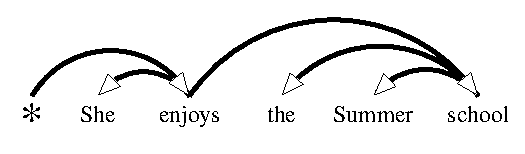
\includegraphics[width=0.6\columnwidth]{figs/parsing/example_proj}
\caption{A dependency tree for the sentence \emph{She enjoys the Summer school}. Note the additional dummy root symbol (*) which is included for convenience.}
\label{fig:deptree_proj}
\end{figure}


\subsection{Projective and Non-projective Parsing}

Dependency trees constructed using the method just described (\emph{i.e.}, lexicalization of context-free phrase-based trees) always satisfy the following properties: 
\begin{enumerate}
\item Each word (excluding the dummy root symbol) has exactly one parent. 
\item The dummy root symbol has no parents.
\item There are no cycles. 
\item The dummy root symbol has exactly one child. 
\item All arcs are \emph{projective}. This means that for any arc $\langle h,m \rangle$, all words in its span (\emph{i.e.}, all words lying between $h$ and $m$) 
are descendents from $h$ (i.e. there is a directed path of dependency links from $h$ to such word). 
\end{enumerate}

Conditions 1--3 ensure that the set of dependency links form a well-formed tree, rooted in the dummy symbol, which spans all the words of the sentence. 
Condition 4 requires that there is a single link departing from the root. 
Finally, a tree satisfying condition 5 is said \emph{projective}: it implies that arcs cannot cross (\emph{e.g.}, we cannot have arcs $\langle h,m \rangle$ and $\langle h',m' \rangle$ 
such that $h < h' < m < m'$). 

In many languages (\emph{e.g.}, those which have free-order) we would like to relax the assumption that all trees must be projective. Even in languages which have fixed word order 
(such as English) there are syntactic phenomena which are awkward to characterize using projective trees arising from the context-free assumption. Usually, 
such phenomena are characterized with additional linguistic artifacts (e.g., traces, Wh-movement, \emph{etc.}). 
An example is the sentence (extracted from the Penn Treebank)
\begin{quote}
We learned a lesson in 1987 about volatility. 
\end{quote}
There, the prepositional phrase \emph{in 1987} should be attached to the verb phrase headed by \emph{learned} (since this is \emph{when} we learned the lesson), 
but the other prepositional phrase \emph{about volatility} should be attached to the noun phrase headed by \emph{lesson} (since the \emph{lesson} was about volatility). 
To explain such phenomenon, 
context-free grammars need to use additional machinery which allows words to be scrambled (in this case, via a movement transformation and the consequent insertion of a trace). 
In the dependency-based formalism, we can get rid of all those artifacts altogether by allowing \emph{non-projective} parse trees. 
These are trees that satisfy conditions 1--3 above, but not necessarily conditions 4 or 5.%
\footnote{It is also common to impose conditions 1--4, in which case the tree need not be projective, but it must have a 
single link departing from the root. The algorithms to be described below can be adapted for this case.} 
The dependency tree in Fig.~\ref{fig:deptree_nonproj} is non-projective: note that the arc $\langle lesson, about \rangle$ is not projective. 

\begin{figure}
\begin{center}
    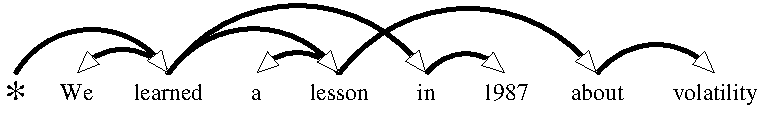
\includegraphics[width=1\columnwidth]{figs/parsing/example_nonproj}
  \caption{A non-projective parse tree.}
  \label{fig:deptree_nonproj}
  \end{center}
\end{figure}

We end this section by mentioning that dependency trees can have their arcs labeled, to provide more detailed syntactic information. 
For example, the arc $\langle enjoys, She \rangle$ could be labeled as {\tt SUBJ} to denote that the modifier \emph{She} has a subject function, and 
the arc $\langle enjoys, school \rangle$ could be labeled as {\tt OBJ} to denote that the modifier \emph{school} has an object function. 
For simplicity, we resort to \emph{unlabeled} trees, which just convey the backbone structure. The cope with the labels, one can use either a joint model 
that infers the backbone and labels altogether, or to have a two-stage approach that first gets the backbone structure, and then the arc labels. 

\subsection{Algorithms for Projective Dependency Parsing}

We now turn our attention to \emph{algorithms} for obtaining a dependency parse tree. 
We start by considering a simple kind of models which are called \emph{arc-factored}.  
These models assign a score $s_{\boldsymbol{\theta}}(h,m)$ to each possible arc $\langle h,m \rangle$ connecting a pair of words; 
they then score a particular dependency tree $t$ by summing over the individual scores of the arcs that are present in the tree: 
$$\mathrm{score}_{\boldsymbol{\theta}}(t) = \sum_{\langle h,m \rangle \in t} s_{\boldsymbol{\theta}}(h,m).$$ 
As usual, from the point of view of the parsing algorithm, 
it does not matter whether the scores come from a generative or discriminative approach, and which features were used to compute the scores. 
The three important inference tasks are: 
\begin{enumerate}
\item Obtain the tree with the largest score, 
$${\hat t} = \argmax_t \mathrm{score}_{\boldsymbol{\theta}}(t).$$
\item Compute the partition function (for a log-linear model),
$$Z(\mathbf{s_{\boldsymbol{\theta}}}) = \sum_t \exp(\mathrm{score}_{\boldsymbol{\theta}}(t)),$$
where $\mathbf{s_{\boldsymbol{\theta}}}$ is short-hand notation for the set of all the $s_{\boldsymbol{\theta}}( h,m )$ coefficients.
\item Compute the posterior marginals for all the possible arcs (which for a log-linear model is the gradient of the log-partition function), 
$$P_{\boldsymbol{\theta}}(\langle h,m \rangle \in t) = \frac{\partial \log Z(\mathbf{s_{\boldsymbol{\theta}}})}{\partial s_{\boldsymbol{\theta}}( h,m )}.$$
\end{enumerate}

\todo{Skip this exercise and write down an optional one at the end asking to implement
Eisner's algorithm given some pseudo-code and evaluate it on English data.}
\begin{exercise}
\textbf{(Warning: this exercise is somewhat complex. Feel free to think about it after the lab and ask your questions later!)}
In \emph{projective} dependency parsing using arc-factored models, the three tasks above can be solved in time $O(N^3)$. 
Sketch how the most likely dependency tree can be computed by ``adapting'' the CKY algorithm. 
(Hint: note that the CKY algorithm builds larger spans by combining smaller spans, 
and multiplies their weights by the weight of the corresponding production rule. 
In dependency parsing, each ``span'' is not represented by a constituent, 
but rather by the position of its lexical head. 
Convince yourself that this can only be either the leftmost or the rightmost position, 
and work out how the two spans can be combined.)

The instantiation of the CKY algorithm for projective dependency parsing is called Eisner's algorithm \citep{Eisner1996}. 
Analogously,  the partition function and the posterior marginals can be computed by 
adapting the inside-outside algorithm. 
\end{exercise}

\subsection{Algorithms for Non-Projective Dependency Parsing}

We turn our attention to \emph{non-projective} dependency parsing. In that case, efficient solutions also exist for the three problems above; 
interestingly, they are based in combinatorial algorithms which are not related at all with dynamic programming: 
\begin{itemize}
\item The first problem corresponds to finding the \emph{maximum weighted directed spanning tree} in a directed graph. 
This problem is well known in combinatorics and can be solved in $O(N^3)$ using Chu-Liu-Edmonds' algorithm 
\citep{Chu1965,Edmonds1967}.%
\footnote{There is a asymptotically faster algorithm by \citet{Tarjan1977} which solves the same problem in $O(N^2)$.} %
This has first been noted by \citet{McDonald2005b}. 
\item The second and third problems can be solved by invoking another important result in combinatorics, the 
\emph{matrix-tree theorem} \citep{Tutte1984}. This fact has been noticed independently by 
\citet{DSmithSmith2007,Koo2007,McDonald2007}. The cost is that of computing a determinant and inverting a matrix, 
which can be done in time $O(N^3)$. 
The procedure is as follows. 
We first consider the directed weighted graph formed by including all 
the possible dependency links $\langle h,m \rangle$ (including the ones departing from the dummy root symbol, 
for which $h = 0$ by convention), along with weights 
given by $\exp(s_{\boldsymbol{\theta}}(h,m))$, 
and compute its 
$(N+1)$-by-$(N+1)$ Laplacian matrix $\boldsymbol{L}$ whose entries are:
\begin{equation}
L_{hm} = \left\{ 
\begin{array}{ll}
\sum_{h'=0}^N\exp(s_{\boldsymbol{\theta}}(h',m)), & \text{if $h=m$,} \\
-\exp(s_{\boldsymbol{\theta}}(h,m))), & \text{otherwise.}
\end{array}\right.
\end{equation}
%Denote by $\boldsymbol{r}=(r_m)_{m=1,\ldots,n}$ the first row of this matrix, transposed, with the first entry removed, i.e., 
%$r_i \triangleq -\exp(s_{\boldsymbol{\theta}}(0,m)))$.
%Furthermore,
Denote by $\hat{L}$ the $(0,0)$-minor of $L$, 
\emph{i.e.}, the matrix obtained from $L$ 
by removing the first row and column. Consider its determinant $\det \hat{L}$ and its 
inverse $\hat{L}^{-1}$. %
Then: %
%% \footnote{The above described is the \emph{multiple root} case, where a valid dependency tree may have multiple words 
%% attached to the dummy root; there is also a solution for 
%% the single root case, where only one effective root is permitted; see \citet{Koo2007}.} %
\begin{itemize}
\item the partition function is given by 
\begin{equation}
Z(\mathbf{s_{\boldsymbol{\theta}}}) = \det \hat{L};
\end{equation}
\item the posterior marginals 
are given by 
\begin{equation}
P_{\boldsymbol{\theta}}(\langle h,m \rangle \in t) = \left\{
\begin{array}{ll}
\exp(s_{\boldsymbol{\theta}}(h,m))\cdot([\hat{L}^{-1}]_{mm} - 
[\hat{L}^{-1}]_{mh}) & \text{if $h \ne 0$}\\
\exp(s_{\boldsymbol{\theta}}(0,m))\cdot[\hat{L}^{-1}]_{mm} & \text{otherwise.}
\end{array}
\right.
\end{equation}
%% $P_{\boldsymbol{\theta}}(\langle h,m \rangle \in t) = 
%% \exp(s_{\boldsymbol{\theta}}(h,m))\cdot([\hat{L}^{-1}]_{mm} - 
%% [\hat{L}^{-1}]_{mh})$, for $h \ne 0$, and 
%% $P_{\boldsymbol{\theta}}(\langle 0,m \rangle \in t) = \exp(s_{\boldsymbol{\theta}}(0,m))\cdot[\hat{L}^{-1}]_{mm}$.
\end{itemize}
\end{itemize}

\begin{exercise}
In this exercise you are going to experiment with arc-factored non-projective dependency parsers. 

The CoNLL-X and CoNLL 2008 shared task datasets \citep{conll06st,Surdeanu2008} contain 
dependency treebanks for $14$ languages. 
In this lab, we are going to experiment with the Portuguese and English datasets. 
We preprocessed those datasets to exclude all sentences with more than 
$15$ words; this yielded the files:
\begin{itemize}
\item {\tt data/deppars/portuguese\_train.conll},
\item {\tt data/deppars/portuguese\_test.conll},
\item {\tt data/deppars/english\_train.conll},
\item {\tt data/deppars/english\_test.conll}.
\end{itemize}

\begin{enumerate}
\item After importing all the necessary libraries, load the Portuguese dataset: 
\begin{python}
import sys
sys.path.append("parsing/" )

import dependency_parser as depp

dp = depp.DependencyParser()
dp.read_data("portuguese")
\end{python}
Observe the statistics which are shown. How many features are there in total?

\item We will now have a close look on the \emph{features} that can be used in the parser. 
Examine the file:
\begin{quote}
{\tt lxmls/parsing/dependency\_features.py}. 
\end{quote}
The following method takes a sentence and computes a vector of features for each possible arc $\langle h, m \rangle$: 
\begin{python}
def create_arc_features(self, instance, h, m, add=False):
	'''Creates features for arc h-->m.'''
\end{python}
We grouped the features in several subsets, so that we can conduct some ablation experiments: 
\begin{itemize}
\item \emph{Basic} features that look only at the parts-of-speech of the words that can be connected by an arc;
\item \emph{Lexical} features that also look at these words themselves;
\item \emph{Distance} features that look at the length and direction of the dependency link (\emph{i.e.}, distance between the two words);
\item \emph{Contextual} features that look at the context (part-of-speech tags) of the words 
surrounding $h$ and $m$. 
\end{itemize}
In the default configuration, only the basic features are enabled. The total number of features 
is the quantity observed in the previous question. 
With this configuration, 
train the parser by running $10$ epochs of the structured perceptron algorithm: 
\begin{python}
dp.train_perceptron(10)
dp.test()
\end{python}
What is the accuracy obtained in the test set? (Note: the shown accuracy is the fraction of words whose parent was correctly predicted.) 

\item Repeat the previous exercise by 
subsequently enabling the lexical, distance and contextual features:
\begin{python}
dp.features.use_lexical = True
dp.read_data("portuguese")
dp.train_perceptron(10)
dp.test()

dp.features.use_distance = True
dp.read_data("portuguese")
dp.train_perceptron(10)
dp.test()

dp.features.use_contextual = True
dp.read_data("portuguese")
dp.train_perceptron(10)
dp.test()
\end{python}
For each configuration, write down the number of features and test set accuracies. 
Observe the improvements obtained when more features were added. 
Feel free to engineer new features!

\item Which of the three important inference tasks discussed above (computing the most likely tree, 
computing the partition function, and computing the marginals) need to be performed in the structured perceptron algorithm? 
What about a maximum entropy classifier, with stochastic gradient descent?  
Check your answers by looking at the following two methods in {\tt code/dependency\_parser.py}:
\begin{python}
def train_perceptron(self, n_epochs):
...

def train_crf_sgd(self, n_epochs, sigma, eta0 = 0.001):
...
\end{python}
Repeat the last exercise by training a maximum entropy classifier, with stochastic gradient descent, 
using $\lambda = 0.01$ and a initial stepsize of $\eta_0 = 0.1$: 
\begin{python}
dp.train_crf_sgd(10, 0.01, 0.1)
dp.test()
\end{python}
Compare the results with those obtained by the perceptron algorithm. 

\item Train a parser for English using your favourite learning algorithm: 
\begin{python}
dp.read_data("english")
dp.train_perceptron(10)
dp.test()
\end{python}
The predicted trees are placed in the file {\tt data/deppars/english\_test.conll.pred}. 
To get a sense of which errors are being made, you can 
check the sentences that differ from the gold standard (see the data in {\tt data/deppars/english\_test.conll}) 
and visualize those sentences, \emph{e.g.}, in 
\url{http://www.ark.cs.cmu.edu/treeviz/}. 

\item (Optional.) Implement Eisner's algorithm for \emph{projective} dependency parsing. 
The pseudo-code is shown as Algorithm~\ref{alg:eisner}. Implement this algorithm as the function
\begin{python}
    def parse_proj(self, scores):
        '''
        Parse using Eisner's algorithm.
        '''
\end{python}
in file ${\tt{dependency\_decoder.py}}$. The input is a matrix of arc scores, whose dimension is 
$(N+1)$-by-$(N+1)$, and whose $(h,m)$ entry contains the score $s_{\boldsymbol{\theta}}(h,m)$. 
In particular, the first row contains the scores for the arcs that depart from the root, 
and the first column's values, along with the main diagonal, are to be ignored (since no arcs 
point to the root, and there are not self-pointing arcs).

To test the algorithm, retrain the parser on the English data (where the trees are actually all
projective) by setting the flag ${\tt{dp.projective}}$ to ${\tt{True}}$:
\begin{python}
dp = depp.DependencyParser()
dp.features.use_lexical = True
dp.features.use_distance = True
dp.features.use_contextual = True
dp.read_data("english")
dp.projective = True
dp.train_perceptron(10)
dp.test()
\end{python}

You should get the following results:
\begin{python}
Number of sentences: 8044
Number of tokens: 80504
Number of words: 12202
Number of pos: 48
Number of features: 338014
Epoch 1
Training accuracy: 0.835637168541
Epoch 2
Training accuracy: 0.922426254687
Epoch 3
Training accuracy: 0.947621628947
Epoch 4
Training accuracy: 0.960326602521
Epoch 5
Training accuracy: 0.967689840538
Epoch 6
Training accuracy: 0.97263631025
Epoch 7
Training accuracy: 0.97619370285
Epoch 8
Training accuracy: 0.979209016579
Epoch 9
Training accuracy: 0.98127569228
Epoch 10
Training accuracy: 0.981320865519
Test accuracy (509 test instances): 0.886732599366
\end{python}

\end{enumerate}
\end{exercise}

\begin{algorithm}[t]
   \caption{Eisner's algorithm for first-order projective dependency parsing\label{alg:eisner}}
\begin{algorithmic}[1]
   \STATE {\bfseries input:} Arc scores $s_{\boldsymbol{\theta}}(h,m)$, for $h \in \{0,\ldots,N\}$, 
   $m \in \{1,\ldots,N\}$, and $h \ne m$, associated with a sentence $s=w_1\ldots w_N$.
   \STATE \COMMENT{Initialization}
	\FOR{$i=0$ {\bfseries to} $N$}
	\STATE \COMMENT{Initialize incomplete spans.}
	\STATE $\mathrm{incomplete}[i,i,\leftarrow] := 0.0$
	\STATE $\mathrm{incomplete}[i,i,\rightarrow] := 0.0$
	\STATE
	\STATE \COMMENT{Initialize complete spans.}
	\STATE $\mathrm{complete}[i,i,\leftarrow] := 0.0$
	\STATE $\mathrm{complete}[i,i,\rightarrow] := 0.0$
	\ENDFOR
	\STATE
	\STATE \COMMENT{Induction}
	\FOR[$k$ is length of span]{$k=1$ {\bfseries to} $N$} 
	\FOR[$s$ is start of span]{$s=1$ {\bfseries to} $N-k$}
	\STATE Set $t := s + k$ \COMMENT{$t$ is end of span}
	\STATE
	\STATE \COMMENT{First, create incomplete spans.}
	\STATE $\mathrm{incomplete}[s,t,\leftarrow] := \max_{s \le r < t} (\mathrm{complete}[s][r][\rightarrow] + \mathrm{complete}[r+1][t][\leftarrow] + s_{\boldsymbol{\theta}}(t,s)) $
	\STATE $\mathrm{incomplete}[s,t,\rightarrow] := \max_{s \le r < t} (\mathrm{complete}[s][r][\rightarrow] + \mathrm{complete}[r+1][t][\leftarrow] + s_{\boldsymbol{\theta}}(s,t))$
	\STATE
	\STATE \COMMENT{Then, create complete spans.}
	\STATE $\mathrm{complete}[s,t,\leftarrow] := \max_{s \le r < t} (\mathrm{complete}[s][r][\leftarrow] + \mathrm{incomplete}[r][t][\leftarrow]$
	\STATE $\mathrm{complete}[s,t,\rightarrow] := \max_{s < r \le t} (\mathrm{incomplete}[s][r][\rightarrow] + \mathrm{complete}[r][t][\rightarrow])$
	\ENDFOR
	\ENDFOR
	\STATE
	\STATE \COMMENT{Termination}
	\STATE Backtrack to obtain the actual tree, whose score is $\mathrm{complete}[0,N,\rightarrow]$.
\end{algorithmic}
\end{algorithm}


\subsection{Model Refinements}

A number of refinements has been made that yield more accurate dependency parsers. We mention just a few: 
\begin{description}
\item[Sibling and grandparent features.] 
The arc-factored assumption fails to capture correlations between pairs of arcs. 
The dynamic programming algorithms for the \emph{projective} case can be extended (at some additional cost) to 
handle features that look at consecutive sibling arcs on the same side of the head 
(\emph{i.e.}, pairs of arcs of the form $\langle h,m \rangle$ and $\langle h,s \rangle$ 
with $h < m < s$ or $h > m > s$, such that no arc $\langle h,r \rangle$ exists with $r$ between $m$ and $s$. 
This has been done by \citet{Eisner1999}. Similarly, grandparents can also be accommodated 
with similar extensions \citep{Carreras2007}. These are called ``second-order models.''

For the non-projective case, however, any extension beyond the arc-factored model becomes NP-hard \citep{McDonald2007}. 
Yet, approximate algorithms have been proposed to handle ``second-order models'' that seem to work well: 
a greedy method \citep{McDonald2006CoNLL}, 
loopy belief propagation \citep{DSmith2008}, a linear programming relaxation \citep{Martins2009ACL}, 
and a dual decomposition method \citep{Koo2010EMNLP}. 
\item[Third-order models.]
For the projective case, third order models have also been considered \citep{Koo2010}. This was 
extended to the non-projective case by \citet{Martins2013ACL}.
\item[Transition-based parsers.]
Like in the phrase-based case, there is a totally different line of work which models parsers as a sequence of greedy 
shift-reduce decisions \citep{Nivre2006CoNLL,Huang2010}. These parsers seem to be very fast (expected linear time) 
and only slightly less accurate than 
the state-of-the-art. Solutions have been worked out for the non-projective case also \citep{Nivre2009}. 
\end{description}

\subsection{External Links}

If you want to check a demo of a parser that use some of the extensions above, you can do so 
at 
\begin{quote}
{\url{http://demo.ark.cs.cmu.edu/parse}} 
\end{quote}
This demo uses  
TurboParser ({\url{http://www.ark.cs.cmu.edu/TurboParser}}), a free software implementation of a fast and accurate dependency parser 
that can parse thousands of tokens per second with state-of-the-art accuracies 
(way faster than the Python implementation that you have used at the labs). 
Feel free to try it at home!

Other well-known software toolkits that implement dependency parsers are:
\begin{itemize}
\item MSTParser ({\url{http://www.seas.upenn.edu/~strctlrn/MSTParser/MSTParser.html}}), a graph-based dependency parser;
\item MaltParser ({\url{http://www.maltparser.org/}}), a transition-based parser;
\item DPO3 ({\url{http://groups.csail.mit.edu/nlp/dpo3/}}), a third-order projective parser;
\item Linear-time dynamic programming parser ({\url{http://acl.cs.qc.edu/~lhuang/}}), a fast transition-based parser.
\end{itemize}








%% \begin{figure}
%% \small
%% \begin{tabular}{ll}
%% (a) 
%% \Tree [.S [.NP [ She ].Pro ] [.VP [ enjoys ].V [.NP [ the ].Det [.Nbar [ Summer ].N [ school ].N ] ] ] ] &
%% (b) 
%% \Tree [.S~(\emph{enjoys}) [.NP~(\emph{she}) [ She ].Pro~(\emph{she}) ] [.VP~(\emph{enjoys}) [ enjoys ].V~(\emph{enjoys}) [.NP~(\emph{school}) [ the ].Det~(\emph{the}) [.Nbar~(\emph{school}) [ Summer ].N~(\emph{Summer}) [ school ].N~(\emph{school}) ] ] ] ] \\
%% (c)
%% \Tree [.enjoys [ ].she [.school [ ].the [ ].Summer ] ] &
%% (d)
%% \begin{tabular}{c}
%% \\
%% 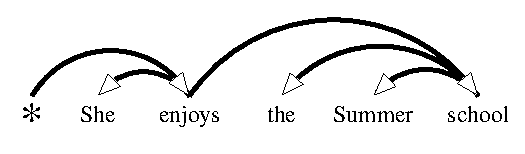
\includegraphics[width=0.55\columnwidth]{figs/parsing/example_proj}
%% \end{tabular}
%% \end{tabular}
%% \end{figure}
